\documentclass{standalone}
\usepackage{tikz}

\begin{document}
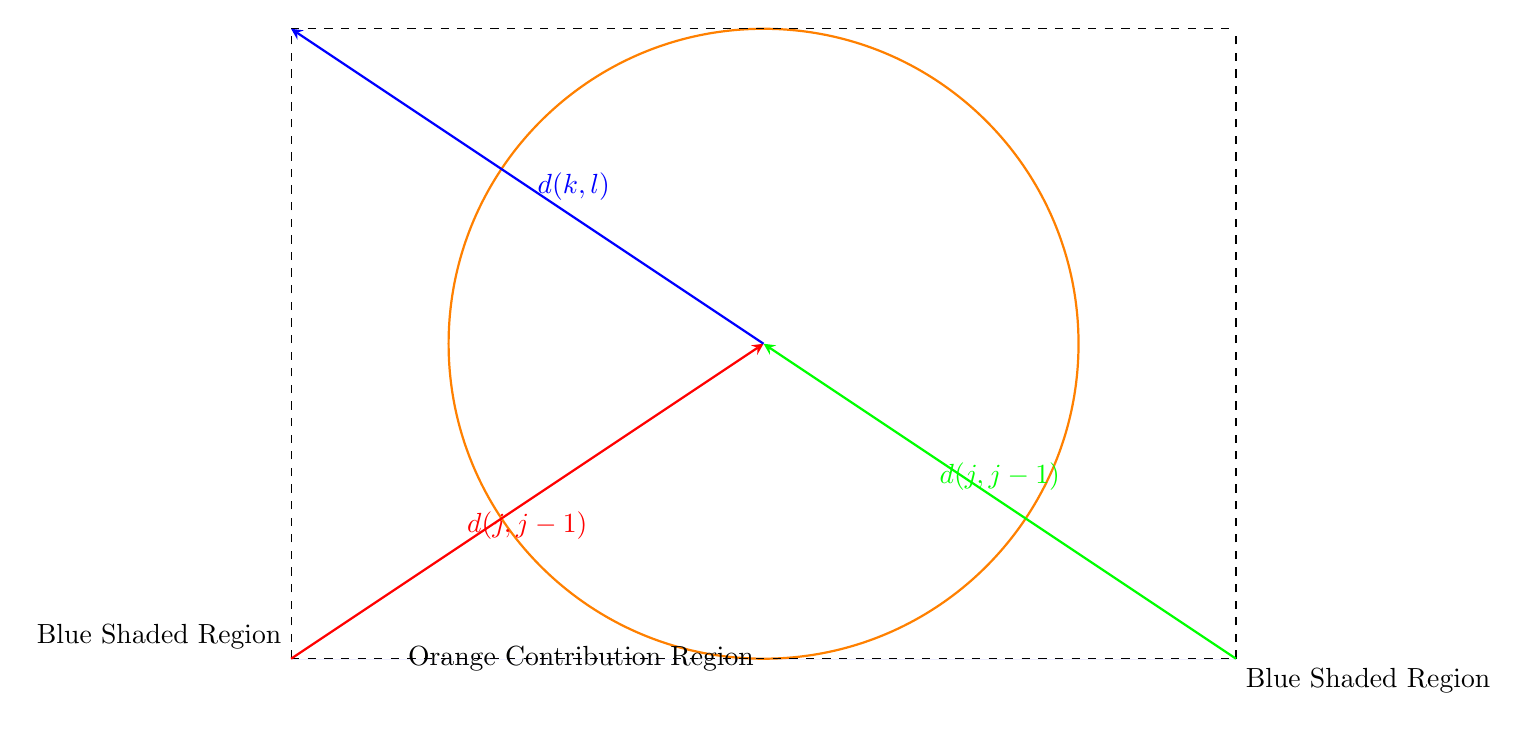
\begin{tikzpicture}[scale=2]
    % Define the coordinates for the regions
    \coordinate (A) at (-3,-2);
    \coordinate (B) at (3,-2);
    \coordinate (C) at (-3,2);
    \coordinate (D) at (3,2);

    % Draw the blue shaded region
    \fill[blue!50] (A) rectangle (B);

    % Draw the orange region
    \draw[orange, thick] (0,0) circle[radius=2];

    % Draw the grid lines
    \draw[dashed] (A) -- (B);
    \draw[dashed] (A) -- (C);
    \draw[dashed] (B) -- (D);
    \draw[dashed] (C) -- (D);

    % Label the regions
    \node[above left] at (A) {Blue Shaded Region};
    \node[below right] at (B) {Blue Shaded Region};
    \node[left] at (0,-2) {Orange Contribution Region};

    % Draw the arrows showing the flow
    \draw[-stealth, thick, red] (A) -- node[midway, below] {$d(j, j-1)$} (0,0);
    \draw[-stealth, thick, green] (B) -- node[midway, above] {$d(j, j-1)$} (0,0);
    \draw[-stealth, thick, blue] (0,0) -- node[midway, right] {$d(k, l)$} (C);
\end{tikzpicture}
\end{document}